\documentclass[tikz,border=2pt]{standalone}
\usepackage{amsmath}
\usepackage{pgfplots}
\pgfplotsset{compat=1.18}

\begin{document}
% Partial sums of 1/n^p: for p=2 they settle (converge to π²/6), for p=1 they keep growing,
% for p=1/2 they grow faster still. The series converges exactly when p>1.
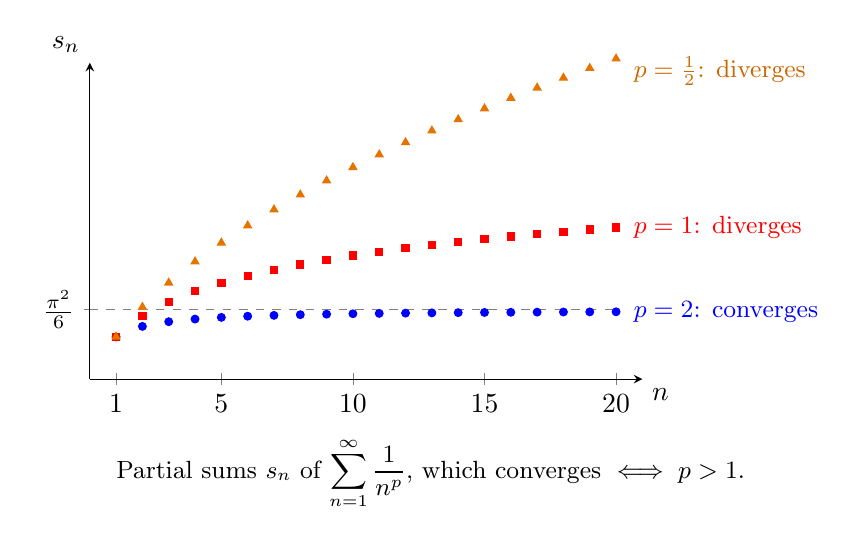
\begin{tikzpicture}
	\begin{axis}[
		axis lines=middle,
		xmin=0, xmax=21,
		ymin=0, ymax=7.5,
		xtick={1,5,10,15,20}, ytick={1.645}, yticklabels={$\tfrac{\pi^2}{6}$},
		xlabel={$n$}, ylabel={$s_n$},
		xlabel style={below right}, ylabel style={above left},
		clip=false,
		width=8.6cm, height=5.6cm
		]
		\addplot[gray, dashed, domain=0:20] {1.6449};
		\addplot[only marks, mark=*, mark size=1.4pt, blue] coordinates {(1,1) (2,1.25) (3,1.3611) (4,1.4236) (5,1.4636) (6,1.4914) (7,1.5118) (8,1.5274) (9,1.5398) (10,1.5498) (11,1.558) (12,1.565) (13,1.5709) (14,1.576) (15,1.5804) (16,1.5843) (17,1.5878) (18,1.5909) (19,1.5937) (20,1.5962)};
		\addplot[only marks, mark=square*, mark size=1.3pt, red] coordinates {(1,1) (2,1.5) (3,1.8333) (4,2.0833) (5,2.2833) (6,2.45) (7,2.5929) (8,2.7179) (9,2.829) (10,2.929) (11,3.0199) (12,3.1032) (13,3.1801) (14,3.2516) (15,3.3182) (16,3.3807) (17,3.4396) (18,3.4951) (19,3.5477) (20,3.5977)};
		\addplot[only marks, mark=triangle*, mark size=1.6pt, orange!90!black] coordinates {(1,1) (2,1.7071) (3,2.2845) (4,2.7845) (5,3.2317) (6,3.6399) (7,4.0179) (8,4.3714) (9,4.7048) (10,5.021) (11,5.3225) (12,5.6112) (13,5.8886) (14,6.1559) (15,6.4141) (16,6.6641) (17,6.9066) (18,7.1423) (19,7.3717) (20,7.5953)};
		\node[blue, anchor=west, font=\small] at (axis cs:20.3,1.6) {$p=2$: converges};
		\node[red, anchor=west, font=\small] at (axis cs:20.3,3.6) {$p=1$: diverges};
		\node[orange!80!black, anchor=west, font=\small] at (axis cs:20.3,7.3) {$p=\tfrac12$: diverges};
	\end{axis}
	\node[anchor=north, align=flush center, text width=10cm, font=\small] at ([yshift=-2pt]current axis.outer south) {Partial sums $s_n$ of $\displaystyle\sum_{n=1}^{\infty}\frac1{n^p}$, which converges $\iff p>1$.};
\end{tikzpicture}
\end{document}
